\documentclass{article}
\usepackage[utf8x]{inputenc}
\usepackage{tikz}

\begin{document}

\section{Drepte distincte}

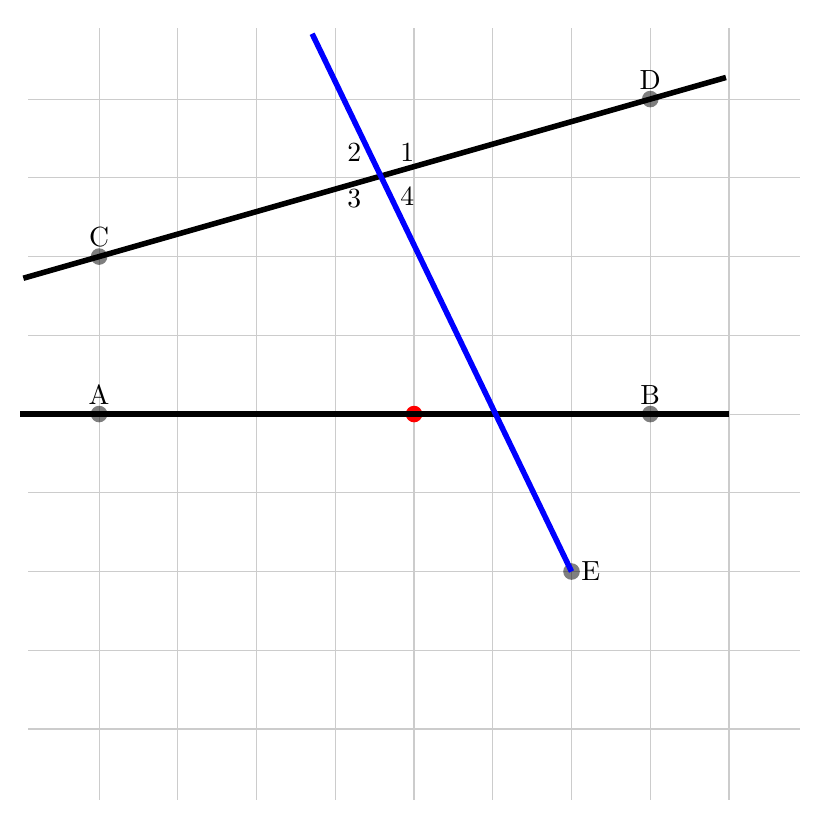
\begin{tikzpicture}[x=1cm,y=1cm]
  % grilă
  \draw[help lines,thin,gray!40] (-4.9,-4.9) grid (4.9,4.9);
  % punctul (0,0) 
  \fill[red] (0,0) circle (3pt);

  % definirea punctelor
  \coordinate[label=A] (A) at (-4,0);
  \coordinate[label=B] (B) at (3,0);
  \coordinate[label=C] (C) at (-4,2);
  \coordinate[label=D] (D) at (3,4); 
  \coordinate[label=right:E] (E) at (2,-2);

  % punctele
  \foreach \point in {A,B,C,D,E}
    \fill [black,opacity=.5] (\point) circle (3pt);

  \draw[line width=2pt, shorten >=-1cm,shorten <=-1cm] (A) -- (B);
  \draw[line width=2pt, shorten >=-1cm,shorten <=-1cm] (C) -- (D);

  % secantă
  \draw[color=blue,line width=2pt] (E) -- (105:5) coordinate (F);
  \coordinate (P1) at (intersection of A--B and E--F);
  \coordinate (P2) at (intersection of C--D and E--F);  

  % pentru a vizualiza punctele de intersecție a secantei 
  % cu dreptele paralele decomentați decomentați următoarele două rînduri
  %\fill [red] (P1) circle [radius=2pt];
  %\fill [red] (P2) circle [radius=2pt];
  
  \node[label=25:1] at (P2) {};
  \node[label=155:2]  at (P2) {};
  \node[label=200:3]  at (P2) {};
  \node[label=-10:4]  at (P2) {};  
\end{tikzpicture}

\textbf{1 Exercițiu:} Marcați cu cifre unghiurile obținute la intersectia secantei cu cealaltă dreaptă.

\newpage

\section{Drepte paralele}

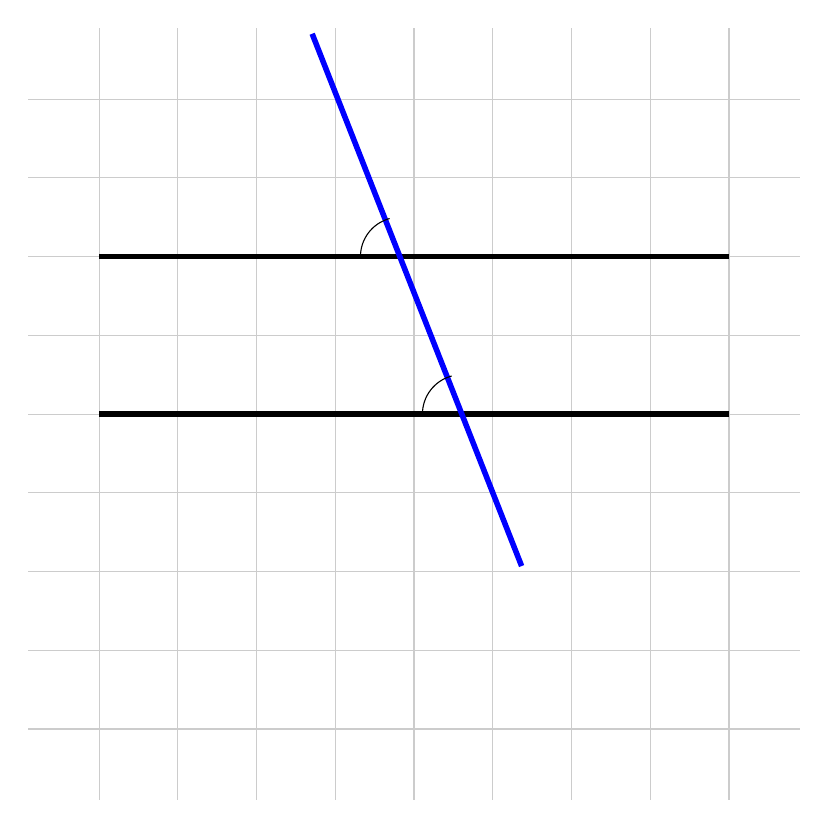
\begin{tikzpicture}[x=1cm,y=1cm]
  % grilă
  \draw[help lines,thin,gray!40] (-4.9,-4.9) grid (4.9,4.9);

  % două drepte parelele
  \draw[line width=2pt] (-4,0) coordinate (a1) -- +(8,0) coordinate (a2);
  \draw[line width=2pt] (-4,2) coordinate (b1) -- +(8,0) coordinate (b2);
  
  % secanta (dusă sub 105 grade față de drepte)
  \draw[color=blue,line width=2pt,shorten <= -1cm] (1,-1) coordinate (s1) -- (105:5) coordinate (s2);
  \coordinate (p1) at (intersection of a1--a2 and s1--s2);
  \coordinate (p2) at (intersection of b1--b2 and s1--s2);  

  % pentru a vizualiza punctele de intersecție a secantei 
  % cu dreptele paralele decomentați decomentați următoarele două rînduri
  %\fill [red] (p1) circle [radius=2pt];
  %\fill [red] (p2) circle [radius=2pt];
  
  \draw ([xshift=-0.5cm]p1) arc (180:105:0.5);
  \draw ([xshift=-0.5cm]p2) arc (180:105:0.5);  
\end{tikzpicture}

\textbf{2 Exercițiu:} marcați unghiurile interne de aceeași parte a secantei.


\end{document}